% This is LLNCS.DEM the demonstration file of
% the LaTeX macro package from Springer-Verlag
% for Lecture Notes in Computer Science,
% version 2.4 for LaTeX2e as of 16. April 2010
%
\documentclass{llncs}
%
\usepackage{makeidx} % allows for indexgeneration
\usepackage{graphicx} % to use \includegraphics{...}
%
\begin{document}
%
\frontmatter % for the preliminaries
%
\pagestyle{headings}  % switches on printing of running heads
\addtocmark{Hamiltonian Mechanics} % additional mark in the TOC
%
\mainmatter % start of the contributions
%
\title{Neural network training with Neuroevolution vs. Backpropagation}
%
\titlerunning{Neuroevolution vs. Backpropagation} % abbreviated title (for running head)
%                                      also used for the TOC unless
%                                      \toctitle is used
%
\author{Thomas Dunajski}
%
\authorrunning{Thomas Dunajski} % abbreviated author list (for running head)

\institute{Hochschule Darmstadt\\
 homepage:
\texttt{https://www.h-da.de/}
}

\maketitle % typeset the title of the contribution

%%
%% The abstract
%%
\begin{abstract}
This work compares the learning speed and accuracy of neuroevolution and backpropagation on automotive data. Neuroevolution of Augumenting Topologies will be compared against Backpropagation using Adaptive Movement Estimation as optimizer. While the training utilizing backpropagation is faster and yields more accurate results, the neuroevolutional approach creates smaller networks and needs less a priori assumptions by the author to learn.
\keywords{Artificial Neuronal Networks, Neuroevolution, Backpropagation, training performance comparison}
\end{abstract}

%%
%% Include all content.
%%
\section{Introduction}
%
Backpropagation (BP) is a well proven approach for training ANNs. It is used in Deep Learning which is the technology powering recent breakthroughs like Alpha Go, the first program that plays Go better than human professionals \cite{Silver.2016}. Neuroevolution (NE) is inspired by how the human brain works [1]. The human brain has over 100 Trillion connections and is a product of evolution. To date it is unmatched when it comes to intelligence. When using Atari games as a benchmark, NE can compete with BP \cite{Salimans.11.03.2017}. It can be scaled to large amounts of CPUs. When using 1000 CPUs it can master 3D humanoid walking within 10 minutes \cite{Salimans.11.03.2017}. Both strategies are used in cutting edge AI research by Google and Open AI. 
%
\subsection{Scope of this work}
Since both approaches have great potential, this work will compare their training performance. The experiments will do a simple regression task on automotive data. After training ANNs with each strategy using the same data, the author will compare how long it took to train them and how good their predictions are on test data. In order to explain the different results the structures of the ANNs will be analyzed. Following that, the learning process itself will be analyzed using data gathered during training.

\section{Foundations}
%
Artificial Neuronal Networks (ANN) are used to solve complex tasks like classification or regression. While Backpropagation (BP) uses a statistical approach to continuously optimize one ANN, Neuroevolution (NE) uses evolutionary tactics to evolve the structure and weights of an entire population of ANNs \cite{Stanley.2002}. 
%
\subsection{Artificial Neuronal Networks}
%
ANNs consist of neurons and connections. The neurons are arranged in layers. Each neuron applies an activation function to its inputs and depending on the result activates its own output or not \cite{Braspenning.1995}. Outputs are connected to inputs of neurons in the next layer. Each output value is multiplied by a weight before being passed to the next neurons input \cite{Braspenning.1995}. During training the weights of connections are optimized until the ANN is capable of solving the problem at hand. To further change the activation behavior of a neuron, biases can be added. A bias neuron has a constant output value and can be connected to a neuron to apply a constant to its activation function.  Information only travels from input to output which is again an input to the next layer. This process is called Forward Propagation \cite{Braspenning.1995}. Other kinds of ANNs like Recurrent Neuronal Networks exist, but are not the focus of this work.
%
\subsection{Backpropagation}
%
The basic concept of training a feed forward ANN using BP is that weights are adjusted depending on how much influence they had in producing an error. This influence is computed by applying the chain rule. The error function is than minimized by performing a gradient descent. Because the influence of a inner neuron is dependent on the neuron(s) in the next layer it is connected to, they have to be evaluated starting with network output moving in the direction of the input. This is the opposite direction than in forward propagation. That is where the name backpropagation comes from \cite{Rojas.1996}.
%
\subsection{Optimizer}
%
The function doing the minimization during training is called optimizer. By applying it every epoch, the weights get adjusted and the error should decrease. The topology of the ANN is fixed and decided on in advance.
%
\subsection{Sigmoid}
%
$$ f (x) =  \frac{\mathrm{1} }{\mathrm{1} + e^{-x} }  $$ 
\newline
The Sigmoid function is one of the most used activation functions [4]. It is differentiable which is a requirement for using it in gradient decent \cite{Rojas.1996}. The derivate of the function can never be 0. This means that the gradient descent will not get stuck before reaching the minimum of the error function \cite{Rojas.1996}.  
%
\subsection{Loss function}
%
A function that is used to determine the difference between the generated output and the expected value is called loss function. Loss functions need to map values to one real value. Repeatedly applying an optimizer to minimize the loss function is how the ANNs learn.
%
\subsection{Adaptive Moment Estimation (ADAM)}
%
Adam is an optimizer function that combines ideas from RMSPRop and ADAGrad. It works well on a large range of problems and performs well on large datasets and/or on large amounts of parameters \cite{Kingma.22.12.2014}. Likewise it performs well on small batch sizes \cite{Kingma.22.12.2014}. It computes individual learning rates for different parameters based on estimated moments of gradients \cite{Kingma.22.12.2014}.
%
\subsection{Neuroevolution }
%
The basic concept is that a population of ANNs is subjected to mutation and crossover. The fittest ANNs make it into the next generation.  This repeated survival of the fittest leads to optimization. While NE can use a wide range of activation functions it needs a suited fitness function \cite{Stanley.2019}.
%
\subsection{Neuroevolution of Augmenting Topologies (NEAT)}
%
In contrast to BP where the topology is decided before the experiment begins, NEAT can evolve the topology at the same time. This can possibly reduce the search space and save training time \cite{Stanley.2002}. NEAT starts with only the inputs and outputs, which are fully connected as starting structure. It than evolves the hidden layers, by inserting and removing nodes and connections. This leads to a minimal structure size that in term reduces training time because of the minimal weight space \cite{Stanley.2002}.  
%
\subsection{Speciation}
%
Speciation is used to protect innovation as inserting new nodes will decrease an ANN’s fitness until its weights had the chance to be optimized \cite{Stanley.2002}. Dividing the population into species and ensuring that some members of new species survive long enough for their weights to adjust, ensures that new topologies are not instantly discarded. 
%
\subsection{Historical Markings}
%
An ID is assigned to each new inserted node or connection. This historical marking is used to determine which species an ANN belongs to and makes crossover possible. To separate the solution candidates into several species, the distance between their historical markings is used. Two genomes with similar markings have a similar topology, as they both are close descendants of a genome in a previous generation \cite{Stanley.2002}. 
%
\subsection{Crossover and Competing Conventions}
%
According to Ken Stanley et al. the Competing Conventions Problem is critical for applying Crossover on two ANNs \cite{Stanley.2002}. The problem is that two identical ANNs might be described differently. Imagine a network with 3 nodes A, B and C with connections from A to B and C (ABC) and another one with the same connections, where B and C swapped places (ACB). Both networks are the same but in a different notation. If a crossover applied to ABC and ACB swaps the last node of each network, we end up with ABB and ACC. Both networks are now broken. NEAT uses the historical markings to solve this problem. During crossover these markings are compared and only nodes or connections with identical markings are allowed to be swapped. This eliminates the need for expansive topology analysis \cite{Stanley.2002}. Crossover is not necessary for NE, but it improves training results \cite{Stanley.2002}.
%
\section{Performance Evaluations}
%
The following experiments evaluate the learning performance of BP and NEAT on a regression task.
%
\subsection{Data }
%
The following experiments use the Auto MPD Data Set from the Carnegie Mellon University. It was released in 1983. The dataset is rather old, but for the purpose of this paper its age is irrelevant. It was chosen for this experiment, because it is compact and comprehensible. It has 398 entries each consisting of 8 attributes. 6 entries have been dropped because they were not complete, leaving 392 to work with. The ANNs will have to estimate the Miles per Gallon (MpG) value associated with Cylinders, Displacement, Horsepower, Weight, Acceleration, Model, Year and Origin of a car model. The origin will be encoded in an one hot encoding (Europe, USA, Japan) meaning that instead of one input with three values there will be three inputs with either 1 or 0 as value. All other attributes are normalized. In order to test the abstraction of the ANNs, 20\% of the entries have been randomly selected as test data and are not used for training.  
%
\subsection{Experiment using Backpropagation }
%
The BP experiment was performed using Tensor Flow. ADAM was used as optimizer. The squared mean error was  used as loss function.  As evaluation metric the mean absolute error is used across all experiments. The maximum epochs were set to 1000. When the validation error started increasing, which is a sign for overfitting, the training was stopped. The ANN consists of two fully connected layers with 64 neurons each. This means that there are a total of 4865 parameters to train within the network.
%
The experiment yielded the following results:
%
\begin{center}
	\begin{tabular}{ | c | c| c | } 
		\hline
		Backpropagation & Validation error & Epochs \\ 
		\hline
		first run & 1.97   & 205 \\ 
		\hline
		second run & 1.92 & 222 \\ 
		\hline
		third run & 1.94 & 194 \\ 
		\hline
		average & 1.94 & 207 \\ 
		\hline
	\end{tabular}
\end{center}
%
Every run reached below 2 MpG error on the training data using mean squared error as loss function and below. For later comparison the following NE experiments will terminate once they reach this error rates during training. The error on the training data and test data is almost identical using BP. This indicates that the ANN has generalized well and can be used for predictions on data not included in the train data set. 
%
\subsection{Experiment using Neuroevolution}
%
The experiment uses exactly the same data as the one using BP. As implementation the NEAT Python framework \cite{AlanMcIntyreandMattKalladaandCesarG.MiguelandCarolinaFeherdaSilva.} is used. It uses a direct encoding with two genomes. One containing the nodes the other containing the connections. It uses historical markings for crossover and speciation to protect innovation. In contrast to BP, no topology has been chosen for the ANN, because finding the topology is part of the learning process. The configuration only uses sigmoid as activation function for comparison with Experiment 1. During training biases can be added to and removed from solution candidates.  All experiments use a population size of 150 solution candidates. The training will be stopped once an ANN is producing the targeted Miles per Gallon mean error. This would mean the results should be quality wise close to the results from the BP experiment above. It is important to note that another criteria would be needed to determine when to stop the experiment if it would not need to reach the same quality of results, like the BP experiment. The best solution makes it into the next generation without modification. This is called elitism and prevents the best solution from getting worse. As fitness function the inverse of the squared mean error was used. That way the loss function in Experiment 1 and the fitness function in Experiment 2 and 3 were almost the same. The inversion was only applied to have growing fitness values. The maximum generations were set to 10000. 
The experiment yielded the following results:
%
\begin{center}
	\begin{tabular}{ | c | c| c | } 
		\hline
		Backpropagation & Validation error & Epochs \\ 
		\hline
		first run & 2.72 & 2831 \\ 
		\hline
		second run & 2.71 & 609 \\ 
		\hline
		third run & 3.00 & 924 \\ 
		\hline
		average & 2,81 & 1455 \\ 
		\hline
	\end{tabular}
\end{center}
%
Although the resulting ANNs reach below 2 MpG error on the training data, they only reach on average 2,81 MpG error on the test data. This can be due to overfitting or due to a lack of generalization. Although this results are not as precise like the ones from Experiment 1 they are within 31\% distance to it. 
\newline
\newline
\begin{center}
	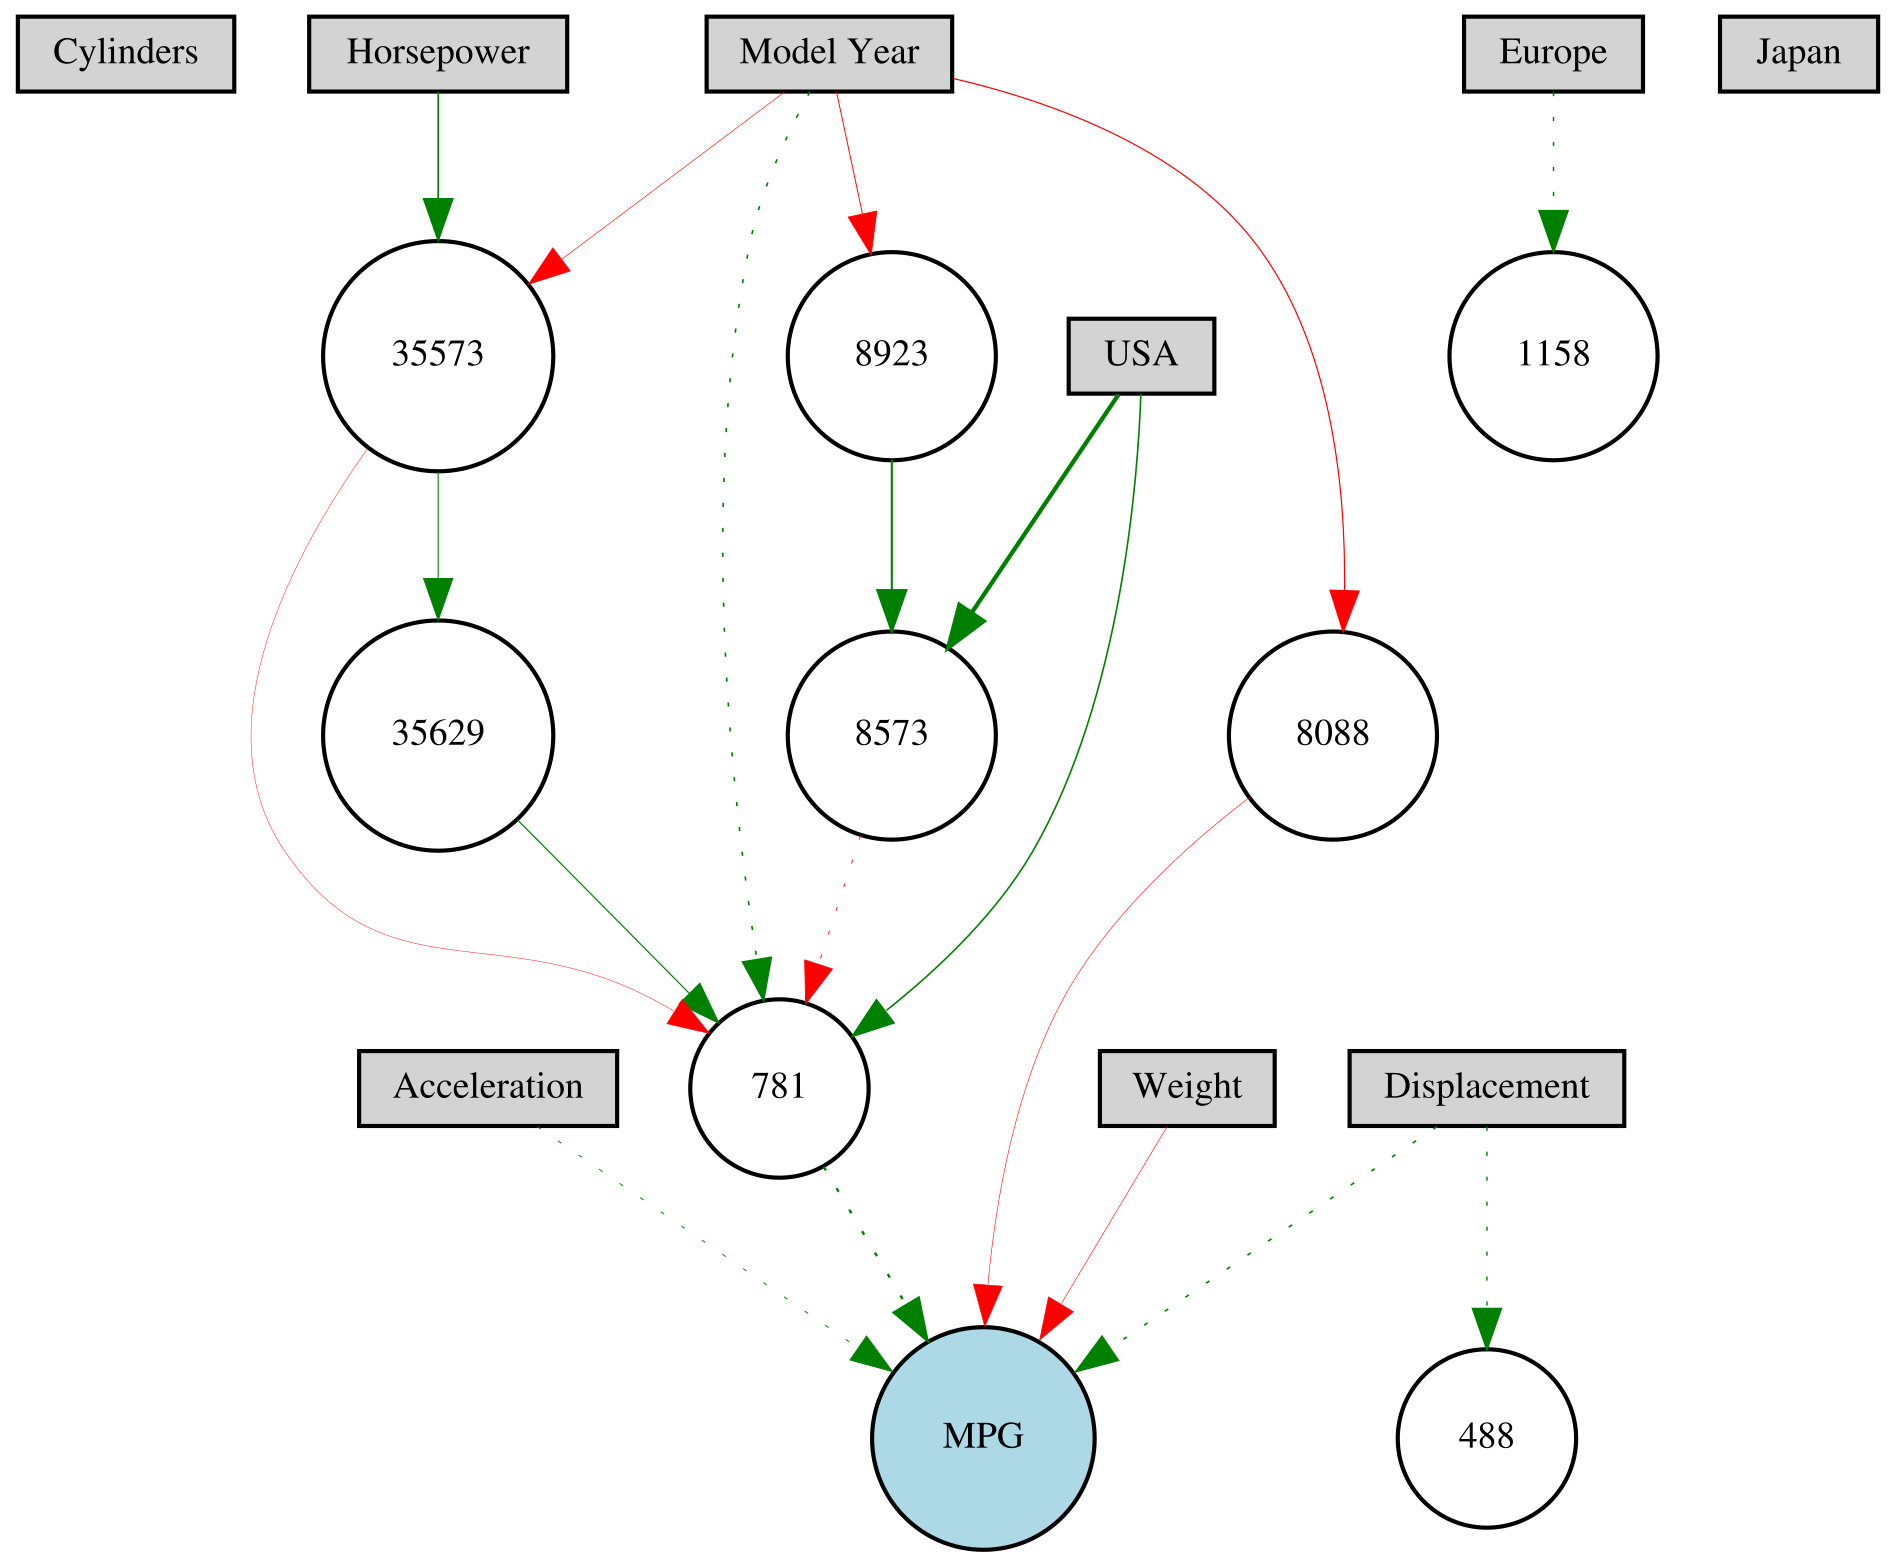
\includegraphics[scale=0.45]{Topologie.png}
	\newline
\end{center}

%
The graph shows one of the ANNs that reached the less than 2 MpG threshold. We can see that not all inputs are used and that some nodes do not connect to the output and can be removed without altering its behavior. Although no two topologies were identical all ANNs that reached below 2 MpG share one trait. They use the weight and model year hinting toward a big influence of these attributes. 
%
\section{Comparing the results}
%
Although the experiments used the same data and the same loss function / fitness function the results were different. This section tries to show the underlying differences in the ANNs and analyze where they come from. 
%
\subsection{Error over time}
%
The first graph shows the average fitness (inverted mean squared error) of the population in blue and the fitness of the best candidate in red (Experiment 2). The second graph shows the mean absolute training error in blue (Experiment 2).
%
\newline

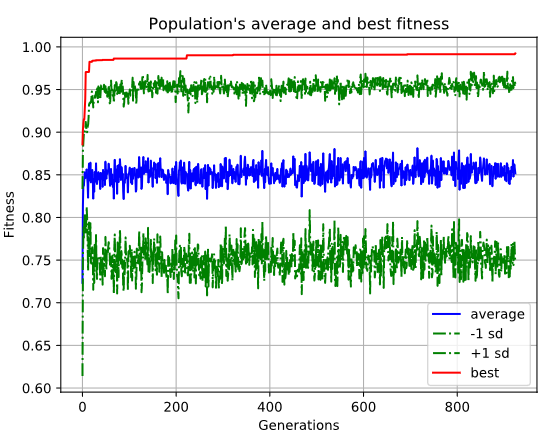
\includegraphics[scale=0.36]{Fitness.png}
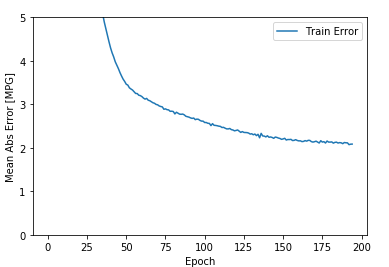
\includegraphics[scale=0.5328]{BP.png}
\newline
\newline
%
While we can see that the BP curve is rather smooth, the NEAT average curve is strongly oscillating. This is because of the high randomness of the evolution. If we look at the red best solution it shows more similarity with the BP curve. Meaning both improve fast in the beginning and slower in later epochs. But while the BP curve shows a trend towards improvement in most epochs, the best solution in NEAT stagnated for long periods.   
%
\subsection{Epochs/Generations needed}
%
The BP experiment terminated in between 158 and 222 epochs. While the amount of generations using NEAT differed widely in different runs, with the fastest ending after 924 and the slowest running one taking 2831 generations to complete. This difference can again be explained with the randomness involved in the evolutional process.
%
\subsection{Network shapes}
%
The network shapes show another key difference. The NEAT experiment produced ANNs with 19 nodes on average. This is way less than the 128 nodes in the BP experiment. The difference is even bigger when we compare the amount of connections. While the BP experiment has more than 4500 connections the ANNs created by the NEAT experiment had an average of 21 connections. This means the NE approach can produce smaller networks that in term run faster, because there are less calculations involved. This could be an advantage on devices with low computing power or devices being powered by a battery like mobile phones where efficiency is important.
%
\section{NEAT with different activation functions}
%
This experiment is identical to the first NEAT experiment, except for one configuration. This time the activation functions are randomly selected from the following functions: Sigmoid, Exponential function, Identity and Square. During training there is a 10\% chance that a mutated candidate will have one of its activation functions replaced by a random one of the mentioned functions. This changed the results dramatically:
%
\begin{center}
	\begin{tabular}{ | c | c| c | } 
		\hline
		Backpropagation & Validation error & Epochs \\ 
		\hline
		first run & 3,12 & 319 \\ 
		\hline
		second run & 2.93 & 221  \\ 
		\hline
		third run & 3.03 & 134  \\ 
		\hline
		average & 3,03 & 245 \\ 
		\hline
	\end{tabular}
\end{center}
%
\subsection{Origin of the performance gains}
%
Because only the activation functions were changed it is safe to assume that the change in performance comes from introducing them. Looking at the image below one can see that the final topologies were similar to the ones in the first experiment. This further solidifies that the different activation functions are the reason for the speed up.
%\newline
\begin{center}
	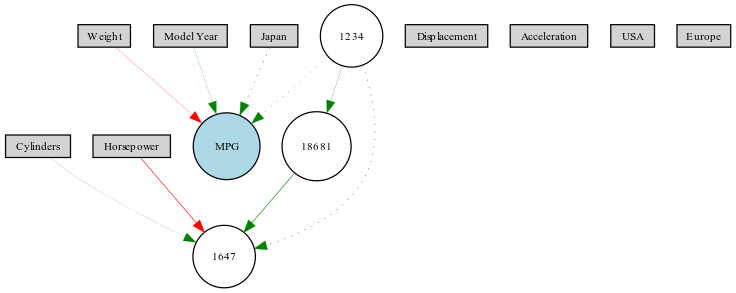
\includegraphics[scale=0.45]{Topologie2.png}
\end{center}
%
It seems that finding weights that satisfy the requirement in mean training error is easier with some activation functions than with other ones. By letting the evolutionary process decide which activation function should be used, the training time needed dropped to on average 38 generations more than with BP. Additionally NEAT supports a larger variety of activation functions, because it can use functions that are not differentiable. NEAT still uses populations of 150 solution candidates, evaluating each one against all training data each generation. But on the other hand the networks are much smaller than the ones generated using BP and there are less parameters to train. Still BP needed less computation measured in generations and real time using the same hardware.

\section{Conclusion}
%
On simple regression tasks BP outperforms NE or at least NEAT, that is representing NE in this work. Training took less computing and did not have much fluctuation in how many epochs were needed. The mean error on the test data was smaller by an average of 31\% when using the same activation function and loss/fitness function. On the other hand the NE approach did need no other input by the author than the fitness function and the amount of inputs and outputs to produce ANNs. While learning is faster and more precise using BP, NEAT explores different topologies and finds minimal solutions, with much fewer neurons and connections. Because it explores the search space with many solution candidates, it can try different approaches in the process and through evolution refine the best ones it finds. 
%
\subsection{Why BP training was faster}
NEAT uses a population of solution candidates and applies random mutations that do not necessarily lead to better results from generation to generation. In each generation all candidates are evaluated against all training data. BP on the other hand uses just one candidate and only iterates once over the training data per generation (epoch). This difference gives BP an advantage when it comes to training time, making NEAT a poor choice to be used on problems where training with BP already needs excessive amounts of computing like Deep Learning. Other variants like HyperNEAT\cite{.18.05.200921.05.2009} that use the same fundamental strategies are better suited to be applied on that kind of problems. Still the conceptual differences between the statistical and evolutionary approaches remain in place. 
\newline
\subsection{Advantages of NEAT}
On the other hand the NEAT approach has its own advantages. It was able to learn without any a priori assumptions by the author except for specifying the amount of inputs, outputs and the fitness function. In the BP experiment two fully connected layers with 64 neurons each have been used to get the results. This has been configured in advance. Without further experiments it is not possible to tell if they were needed, or if 50 neurons per layer would have been sufficient. The same is true for the amount of layers. One has to decide in advance how many layers are needed. This can be a disadvantage because before the training started, it is already decided how many nodes and connections can be modified by the training process. Additionally NEAT can add other sources of innovation during training like recurrent connections. Like recurrent connections these can be inserted at random and the evolutionary process decides if they survive depending on the resulting fitness. Another thing NEAT could introduce to an ANN are nodes with different activation functions. For example nodes with the sin(x) function as activation function could prove useful in data with oscillating patterns like solar power production, that depends on the day and night cycle. Experiment 3 showed significant improvements by intorducing new activation functions. In order for the resulting ANNs to be better comparable between Neat and BP, neither recurrent connections nor different activation functions have been used in the second experiment. 

%
\subsection{Interpreting the experiment results}
  Although the experiments in this work indicate that for regression task with small data sizes BP should be preferred, this is not a conclusion that can be drawn, because the NE experiments were designed to match the training error of the BP experiment, not to produce the best possible results. 
%
%
\section{Discussion and Future Work}
%
Testing learning performance on variety of datasets would be a good next step, because the experiments used a small data set and the results might change on different datasets. NE is performing well in reinforcement learning tasks where agents have to learn from trial and error without any help \cite{Stanley.2019}. Comparing BP and NE strategies in this field is an obvious direction for future research \cite{Salimans.11.03.2017}.  
\newline
Bringing ideas from BP and NE together and creating hybrids of the strategies might be very interesting as well. I.e. generating a topology using NEAT or one of its brethren in a first step and then using BP on the topology might lead to a minimal network size seen in the NEAT experiment and the precision seen in the BP experiment. Another type of hybrid approach might be combining both approaches during learning, i.e. use BP on each solution candidate to train its weights and using the training error as fitness value \cite{Desell.16.03.2017}. 
%
%
\newline
\newline
\newline
Sourcecodes can be found on https://github.com/ThomasDunajski/Neuroevolution-vs-Backpropagation-paper
%
% ---- Bibliography ----
%



%%
%% Include external BibTex data.
%%
\bibliographystyle{./splncs03}
\bibliography{./quellen}

%%
%% The End.
%%
\end{document}
